\chapter{Introduction}\label{ch:Introduction}

\gnote{pull energy, population references from Brunner thesis, point to Chen's fusion energy book, Wesson?}
The population of the earth is projected to increase substantially over the next half-century, potentially reaching as high as 10 billion globally by 2050.  At the same time, any attempt to increase the quality of life of the existing population will necessarily involve increased energy consumption per capita, with a greater fraction of the earth approaching ``first-world'' consumption levels \note{find refs for both}.  As such, worldwide energy consumption will likely continue to increase in the next few decades \note{BP refs for projections from Brunner?}

This increase in energy demand occurs in parallel with increased pressure on traditional energy sources.  Fossil fuels (oil, coal, and natural gas), while reliable sources of base-load power, nevertheless face issues.  Oil faces increasing cost and technical difficulty in capturing dwindling available reserves, as well as the potential for serious ecological damage from accidents (\eg the Deepwater Horizon offshore rig accident in 2010).  Coal, while more readily available \note{cite for estimates of coal stores in the US}, releases particulate matter into the atmosphere, with serious consequences both to the environment and to human health, as well as the greenhouse gases tied to deleterious climate change.  

Renewable energy sources have a certain ``green'' appeal, but each is subject to strict limitations on their implementation.  Solar and wind power suffer from a large degree of variability in their output, necessitating a combination of expensive energy storage methods or (often fossil-fuel based) backup production to handle shortfalls.  Hydroelectric and geothermal power are suitable for base-load power production, but are strictly restricted in their implementation by geographic concerns -- bluntly, there are relatively few locations where hydro or geothermal power generation is possible, and many of these have already been developed \note{cite for this?}.

Conventional -- that is, fission-based -- nuclear power can also supply carbon-free base-load power, with fuel reserves lasting through the next century.  While nuclear power does  suffer from the potential for extremely serious accidents (Fukushima, Chernobyl) it is, in general, highly safe.  However, public perception of nuclear power hinges on these safety concerns, limiting the expansion of nuclear power to meet increasing demand and the safe long-term handling of existing nuclear waste, as well as, ironically, preventing the replacement of an aging reactor fleet with newer, safer designs.

\emph{Fusion}, the nuclear process driving stellar cores, is a potentially highly attractive option for satisfying the world's growing energy needs in an efficient, environmentally-sound manner.  A fusion reactor would supply base-load power using only a small amount of an effectively inexhaustible fuel (readily available for harvesting from seawater), with no greenhouse gas emissions or meaningfully radioactive waste, and the physical impossibility of a major ``meltdown'' accident.  However, fusion remains in the experimental stage, with significant technical hurdles remaining before the development of a prototype fusion power plant.  This thesis will attempt to contribute to the understanding of one of these hurdles, regarding the requirement for efficient plasma behavior in a reactor scenario \note{reword this!}  Further reading on the development of fusion energy is available to the interested reader in several excellent references. \note{cite Freidberg, Chen, Wesson} \nicesectionending

%%%%%%%%%%%%%%%%%%%%%%%%%%%%%%%%%%%%%%%%%%%%%%%%%%%%

\section{Plasmas for Fusion}\label{sec:intro_plasmas}

A \emph{plasma} is a gas to which sufficient energy has been applied to strip some or all of the electrons off the nuclei of its constituent atoms.  These ions and electrons freely interact with one another, behaving as coupled fluids.  Plasmas of interest for fusion research are comprised of light elements (typically Hydrogen or Helium), and are at extremely high temperatures, in excess of 100 million Kelvin ($10-20 \;\si{keV}$).  As these conditions are far in excess of the ionization energy for these elements, the plasma is dominated by collisions between its charged particles, rather than interactions with bound electron states.

\subsection{Plasma Parameters}\label{subsec:intro_params}

As the plasma is comprised of free charged particles, it responds strongly to electric and magnetic fields.  In the presence of a DC electric field (externally applied, or generated by an imbalance of positive and negative charge in the plasma), the plasma will rearrange itself to screen out the field.  This effect breaks down at short length scales, at which there is an insufficient number of charge carriers to rearrange and counter the field -- the characteristic scale for this effect is the Debye Length, given by

\begin{equation}\label{eq:debye}
 \lambda_D = \sqrt{ \frac{\varepsilon_0 T}{n e^2} }
\end{equation}

\noindent At size scales significantly larger than $\lambda_D$, this will enforce an approximately balanced electric charge in the plasma, termed ``quasi-neutrality''.  This is reflected in the number densities of electrons and multiple ion species $j$, each with charge $Z_j$, by the relation

\begin{equation}\label{eq:quasineutral}
 n_e = \sum_j{n_j Z_j}
\end{equation}

\noindent In a multiple-ion species plasma, we may also define an effective ion charge

\begin{equation}\label{eq:Zeff}
 Z_{eff} = \frac{1}{n_e} \sum_j{n_j Z_j^2}
\end{equation}

The electrostatic force driving this charge redistribution induces a ``ringing'' oscillation in the plasma, at the characteristic plasma frequency $\omega_p$:

\begin{equation}\label{eq:omegap}
 \omega_p = \sqrt{ \frac{ne^2}{\varepsilon_0 m_e} }
\end{equation}

\noindent This natural oscillation in the plasma also has the effect of screening AC electric fields varying at frequencies $\omega < \omega_p$.

Coulomb collisions between charged particles in the plasma tend to drive magnetically-confined plasmas into thermal equilibrium, with the velocity distribution for a species given by the Maxwellian

\begin{equation}\label{eq:maxwell}
 f(v) = n \left( \frac{m}{2\pi T} \right)^{3/2} \mbox{exp}\left(-\frac{mv^2}{2T} \right)
\end{equation}

\noindent These collisions also cause the plasma to emit a continuous spectrum of Bremsstrahlung radiation.  For a plasma in thermal equilibrium, integration over the full spectrum gives for the total radiated power

\begin{equation}\label{eq:brems}
 P_{Brems} = \left( 5.35 \times 10^{-37} \right) n_e^2 Z_{eff} \sqrt{T}
\end{equation}

\noindent representing a consistent source of heat loss from the plasma. \nicesectionending

\subsection{Fusion Fuels}\label{subsec:intro_fuels}

Fusion collectively refers to the class of nuclear reactions merging lighter nuclei into a single heavier element.  While fusion reactions for elements lighter than iron are generally exothermic, as they form nuclei with greater binding energy per nucleon (see Figure~\ref{fig:bindingenergy}), the most common and readily attainable involve isotopes of hydrogen or helium, the most promising candidates for which are shown below.

\begin{align}
 {}^2\si{D} + {}^2\si{D} &\rightarrow {}^3\si{T} + \si{p} + 4.03 \;\si{\mega\electronvolt}\label{eq:dd1}\\
 {}^2\si{D} + {}^2\si{D} &\rightarrow {}^{3}\si{He} + \si{n} + 3.27 \;\si{\mega\electronvolt}\label{eq:dd2}\\
 {}^2\si{D} + {}^3\si{He} &\rightarrow {}^4\si{He} + \si{p} + 18.3 \;\si{\mega\electronvolt}\label{eq:dhe3}\\
  {}^2\si{D} + {}^3\si{T} &\rightarrow {}^4\si{He} + \si{n} + 17.6 \;\si{\mega\electronvolt}\label{eq:dt}
\end{align}

\noindent Here $\si{D}$ and $\si{T}$ indicate nuclei of deuterium and tritium, two heavy isotopes of hydrogen (one proton plus one and two neutrons, respectively).  The fusion reaction rate $R_f$ is given by

\begin{equation}\label{eq:rate}
 R_f = n_1 n_2 \langle \sigma v \rangle_{1,2}
\end{equation}

\noindent where $n_1$ and $n_2$ indicate the densities of the two fuel ions (\eg for deuterium-tritium fuel $n_1 n_2 = n_D n_T$, while for pure-deuterium fuel $n_1 n_2 = \frac{1}{2} n_D^2$ to remove double-counting of fuel ions) and $\langle \sigma v \rangle_{1,2}$ is a rate parameter incorporating the energy-dependent reaction cross-section averaged over the Maxwellian fuel distribution (eqn.~\ref{eq:maxwell}).  In practice, the energy-dependent cross-section is empirically determined -- measured rate parameters $\langle \sigma v \rangle$ for the fuels of interest are shown in Figure~\ref{fig:xsection}.

% \begin{figure}[h]
%  \pushtooutside
%  \fcapside[70mm]{\caption{Binding energy per nucleon versus atomic mass number, with notable isotopes marked.  Reactions forming nuclei with higher binding energy per nucleon are exothermic -- thus, fusion of elements lighter than $\si{Fe}^{56}$ or fission of elements heavier than $\si{Fe}^{56}$ releases energy.}\label{fig:bindingenergy}}{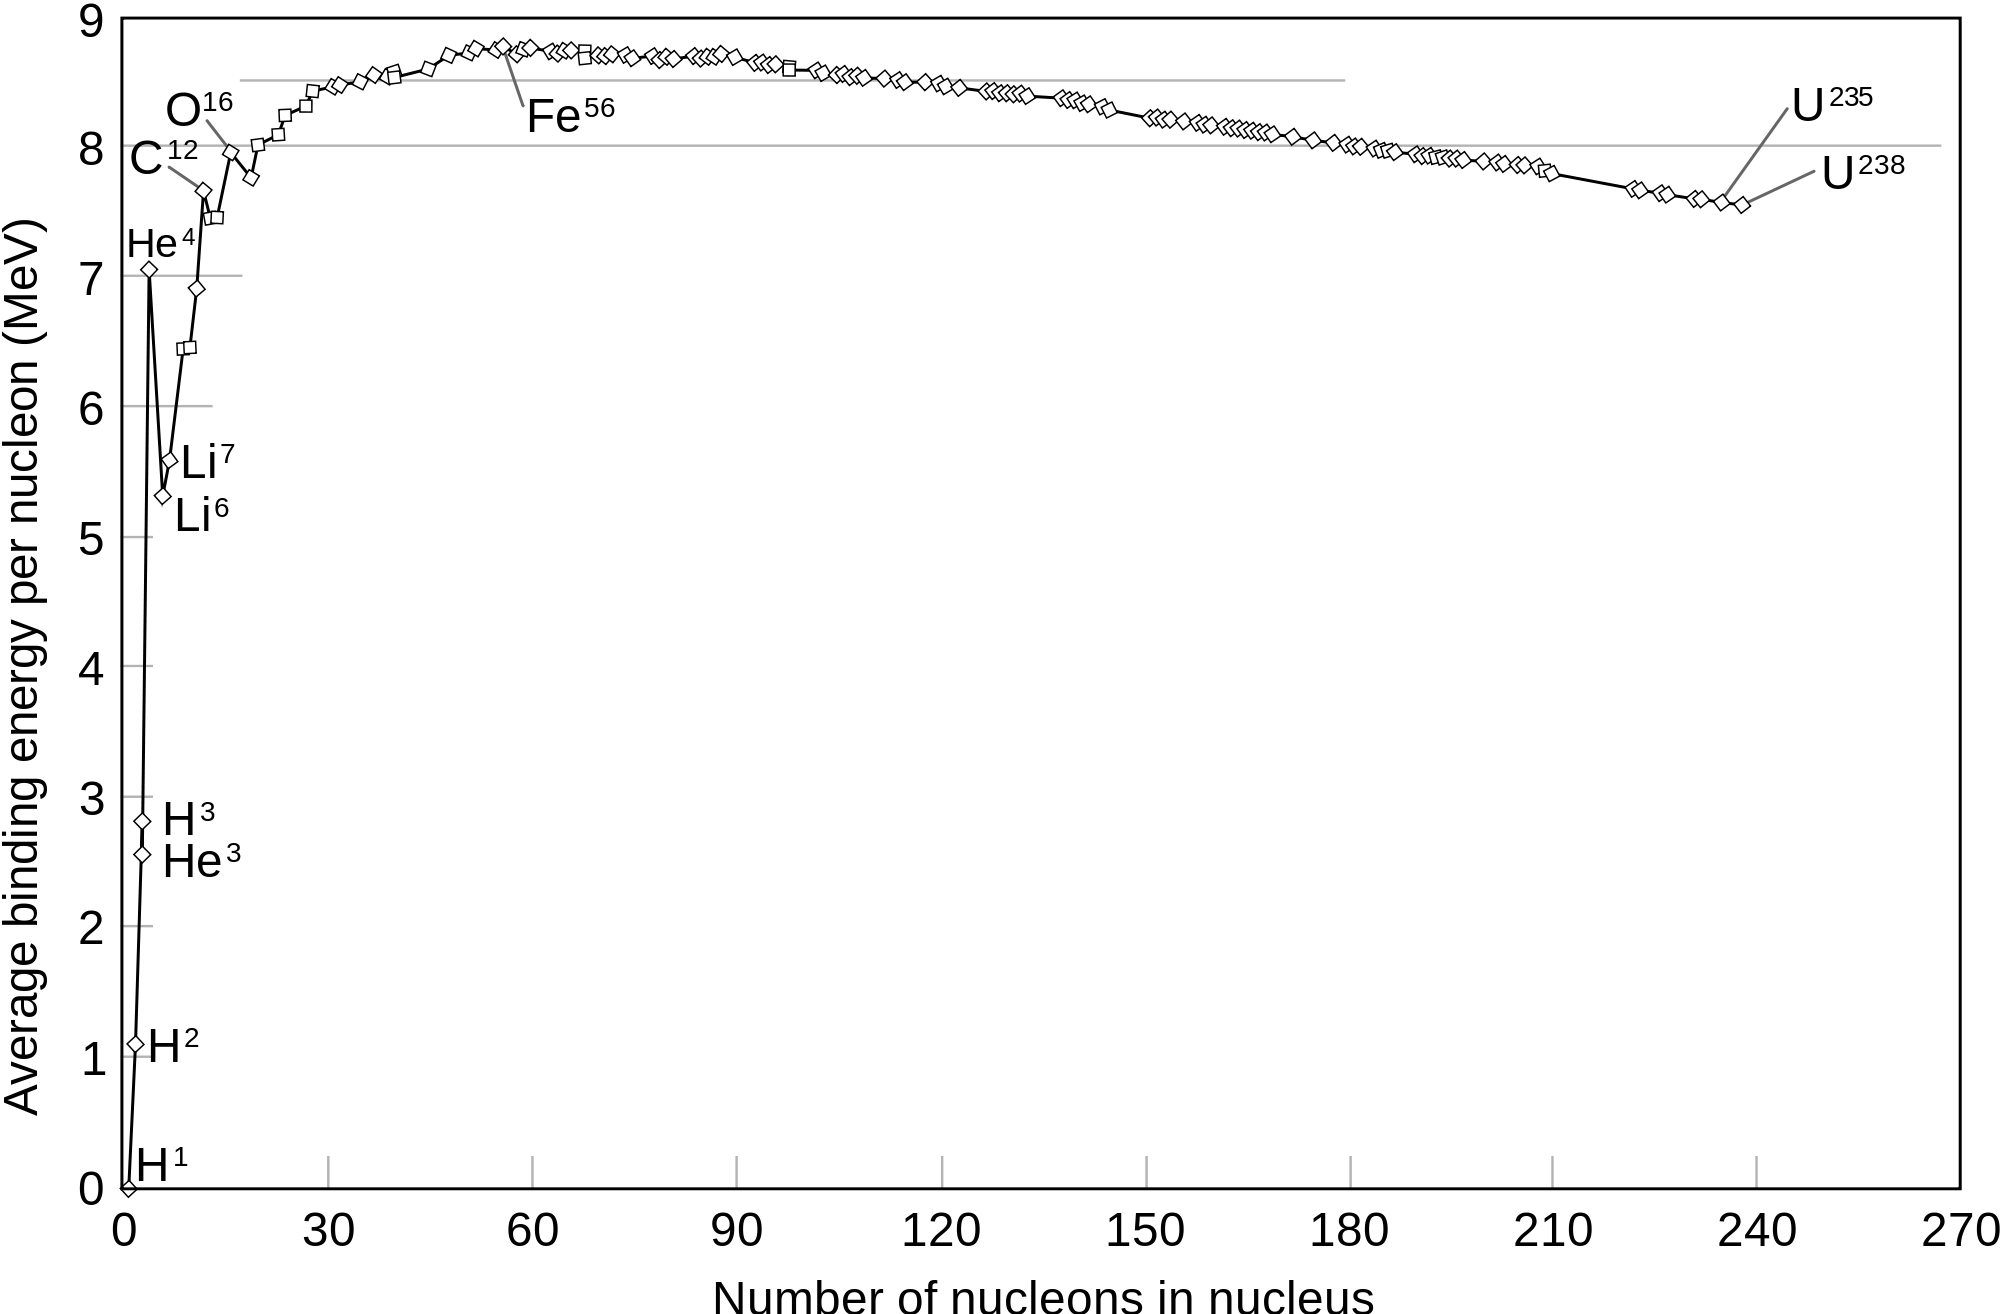
\includegraphics[width=95mm]{graphics/Introduction/bindingenergy.png}}
% \end{figure}
% 
% \begin{figure}[h]
%  \pushtooutside
%  \fcapside[70mm]{\caption{Reaction rate normalized to fuel density for fusion fuels as a function of temperature.  Notably, deuterium-tritium fusion exhibits a higher peak reaction rate, as well as reaching that peak at a lower temperature, than other fuels.}\label{fig:xsection}}{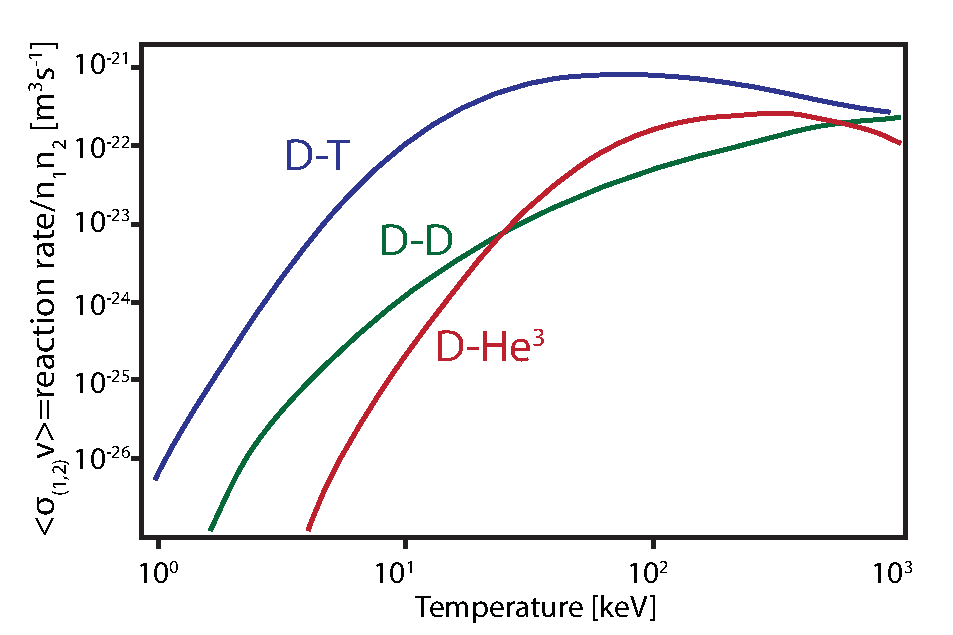
\includegraphics[width=95mm]{graphics/Introduction/reaction_xsections.pdf}}
% \end{figure}

\begin{figure}
 \pushtooutside
 \ffigbox[\FBwidth]{\caption{Binding energy per nucleon versus atomic mass number, with notable isotopes marked.  Reactions forming nuclei with higher binding energy per nucleon are exothermic -- thus, fusion of elements lighter than ${}^{56}\si{Fe}$ or fission of elements heavier than ${}^{56}\si{Fe}$ releases energy.}\label{fig:bindingenergy}}{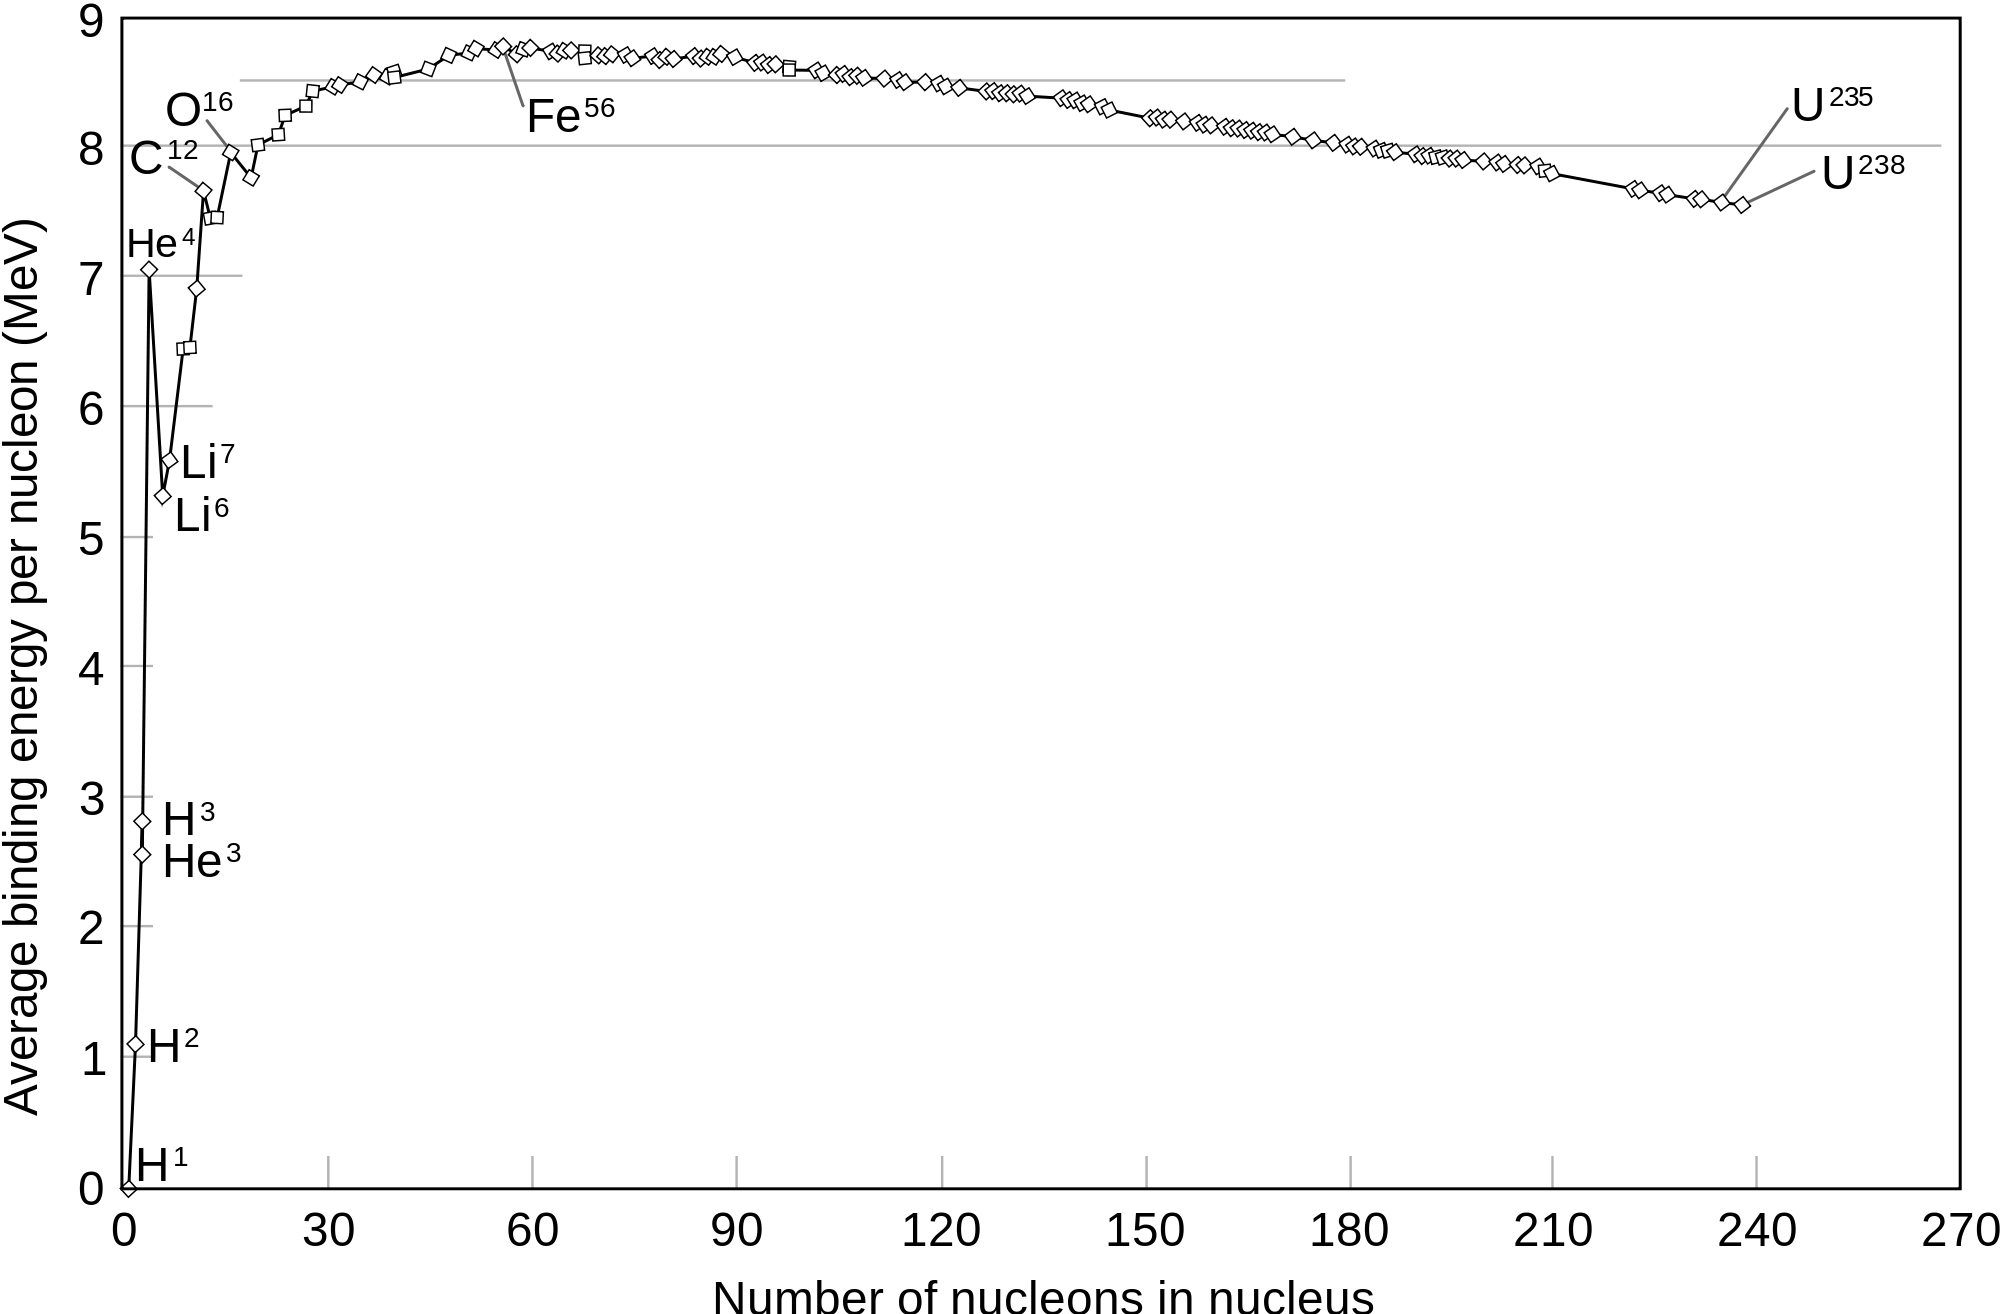
\includegraphics[width=150mm]{graphics/Introduction/bindingenergy.png}}
\end{figure}

\begin{figure}
 \pushtooutside
 \ffigbox[\FBwidth]{\caption{Reaction rate normalized to fuel density, expressed as the rate coefficient $\langle \sigma v \rangle$, for fusion fuels as a function of temperature.  Notably, deuterium-tritium fusion exhibits a higher peak reaction rate, as well as reaching that peak at a lower temperature, than other fuels.}\label{fig:xsection}}{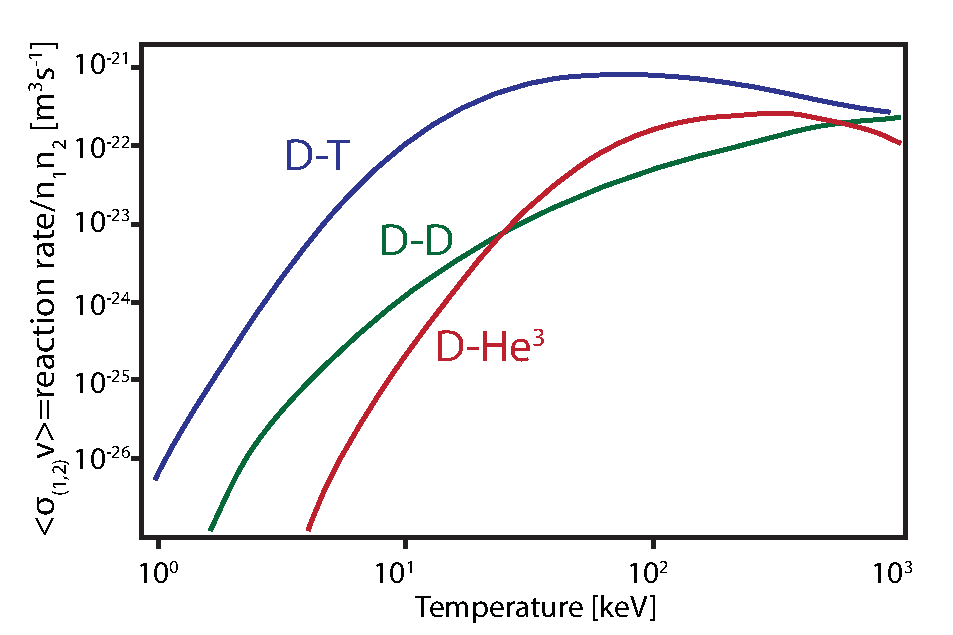
\includegraphics[width=150mm]{graphics/Introduction/reaction_xsections.pdf}}
\end{figure}

Pure deuterium fuel (reactions shown in eqns. \ref{eq:dd1} and \ref{eq:dd2}) is attractive from a research standpoint, due to the abundance and ease of use of deuterium.  Deuterium is a stable nucleus, obviating the need for radiation safety in the fuel system, and is naturally occurring in relative abundance (approximately $1/6000$ of hydrogen nuclei on earth are deuterium \note{cite}), allowing harvesting of deuterium fuel from seawater.  However, pure-deuterium reactions suffer from low energy output per reaction and a significantly lower reaction rate at feasible plasma conditions compared to other fuel options (see Figure~\ref{fig:xsection}), setting high performance requirements for a putative DD-burning reactor.

The $\si{D}-\si{He}^3$ reaction (eqn.~\ref{eq:dhe3}) exhibits several desirable properties, namely an impressive energy yield per reaction, and the fact that the reaction produces only charged particles rather than the high-energy neutrons found in $\si{D}-\si{D}$ and $\si{D}-\si{T}$ reactions, which can cause significant damage to reactor materials.  However, as with $\si{D}-\si{D}$ fuel, the $\si{D}-\si{He}^3$ reaction suffers from a lower reaction rate at attainable conditions, as well as the fact that Helium-3 does not occur in economically usable quantities on Earth.  While off-planet sources of Helium-3 exist (for example, a useful quantity is present in the lunar regolith \note{cite}), this fuel remains the subject of speculation.

The deuterium-tritium reaction (eqn.~\ref{eq:dt}) is considered the most promising for a first-generation fusion reactor, due to its high energy output per reaction and favorable reaction cross-section -- the rate parameter $\langle \sigma v \rangle_{DT}$ reaches its peak at a lower temperature, and reaches a greater absolute level than other fusion fuels.  However, $\si{D}-\si{T}$ operation is limited both by fuel sources, and reaction products.  $\si{D}-\si{T}$ fusion produces a $14 \;\si{MeV}$ neutron, carrying roughly 80\% of the energy released by the fusion reaction, which can damage unshielded reactor materials.  Moreover, while deuterium is stable and readily available, tritium is radioactive with a short half-life (roughly 12.3 years), so it is not naturally occurring in meaningful quantities on earth.   A reactor will solve both of these problems with a \emph{neutron blanket}, a neutron-absorbing structure surrounding the plasma.  This provides the necessary shielding for sensitive reactor 
components.  The heat generated in the blanket from neutron absorption will also be drawn off in a steam cycle to drive turbines, generating electricity from the reactor.  Finally, seeding the blanket with lithium allows the following reactions with fusion neutrons:

\begin{align}
 {}^6\si{Li} + \si{n}_{slow} &\rightarrow {}^4\si{He} + \si{T} + 4.8 \;\si{MeV}\label{eq:Li6}\\
 {}^7\si{Li} + \si{n}_{fast} &\rightarrow {}^4\si{He} + \si{T} + \si{n} - 8.7 \;\si{MeV}\label{eq:Li7}
\end{align}

\noindent the Lithium-6 reaction (eqn.~\ref{eq:Li6}) absorbs ``slow'' neutrons (that is, neutrons that have thermalized to the blanket temperature via collisions) to produce tritium, plus additional heat.  Lithium-7 (eqn.~\ref{eq:Li7}) is more likely to capture fast neutrons to produce tritium in an endothermic reaction; however, the reaction also acts as a neutron multiplier, as a free neutron is maintained through the reaction.  Using blankets enriched with ${}^6\si{Li}$, coupled with neutron multipliers, a reactor will target an over-unity tritium breeding ratio, with $>1$ tritons produced per neutron entering the blanket (\ie per tritium consumed in a fusion reaction).\nicesectionending

%%%%%%%%%%%%%%%%%%%%%%%%%%%%%%%%%%%%%%%%%%%%%%%%%%%%

\section{Magnetic Confinement}\label{sec:intro_magnetic}

\subsection{Basic Principles}\label{subsec:intro_basic}

The temperatures in excess of 100 million Kelvin necessary for fusion in a plasma are inconsistent with any contact between solid reactor materials and the hot core of the plasma.  Magnetic confinement relies on the strong response of the charged particles comprising the plasma to magnetic fields, rather than a material wall, to retain the thermal pressure ($\sim 10 \;\si{atm}$ for a reactor) from the plasma.  The response of a charged particle to electric and magnetic fields is governed by the Lorentz force, \cite{Freidberg2007}

\begin{equation}\label{eq:lorentz}
 \vec{F} = q\left(\vec{E} + \vec{v} \times \vec{B}\right)
\end{equation}

\begin{figure}
 \pushtooutside
 \fcapside[50mm]{\caption{Electron and ion gyro orbits in an applied magnetic field.}\label{fig:intro_gyro}}{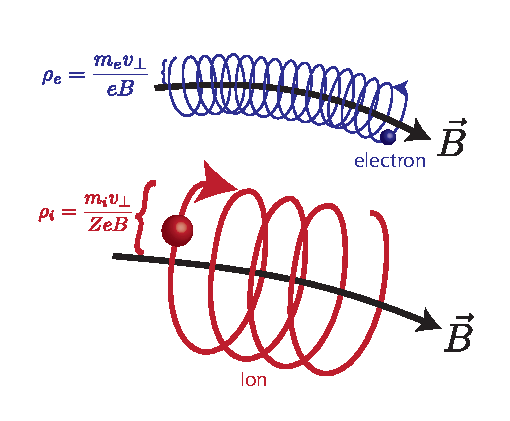
\includegraphics[width=85mm]{graphics/Introduction/gyro.pdf}}
\end{figure}

\subsection{Toroidal Configurations}\label{subsec:intro_toroidal}

%%%%%%%%%%%%%%%%%%%%%%%%%%%%%%%%%%%%%%%%%%%%%%%%%%%%

\section{Alcator C-Mod}\label{sec:intro_cmod}

%%%%%%%%%%%%%%%%%%%%%%%%%%%%%%%%%%%%%%%%%%%%%%%%%%%%

\section{Confinement \& Transport}\label{sec:intro_confinement}

\subsection{Global Confinement}\label{subsec:intro_global}

\subsection{Transport Barriers}\label{subsec:intro_barriers}

%%%%%%%%%%%%%%%%%%%%%%%%%%%%%%%%%%%%%%%%%%%%%%%%%%%%

\section{High-Performance Regimes}\label{sec:intro_regimes}

\subsection{ELMy H-Mode}\label{subsec:intro_elmy}

\subsection{EDA H-Mode}\label{subsec:intro_EDA}

\subsection{I-Mode}\label{subsec:intro_imode}

%%%%%%%%%%%%%%%%%%%%%%%%%%%%%%%%%%%%%%%%%%%%%%%%%%%%

\section{Goals \& Outline}\label{sec:intro_outline}


%%%%%%%%%%%%%%%%%%%%%%%%%%%%%%%%%%%%%%%%%%%%%%%%%%%%

% do per-chapter bibliographies, or one big one?
\bibliographystyle{plainurl}
\bibliography{../references} 